\documentclass[11pt,a4paper]{article}

% ---------------------------------------------------------------------------
%  Packages
% ---------------------------------------------------------------------------
\usepackage[margin=1in]{geometry}
\usepackage[utf8]{inputenc}
\usepackage[T1]{fontenc}
\usepackage{lmodern}
\usepackage{amsmath}
\usepackage{graphicx}
\usepackage{xcolor}
\usepackage{booktabs}
\usepackage{listings}
\usepackage{enumitem}
\usepackage{parskip}
\usepackage{tikz}
\usetikzlibrary{shapes.geometric, arrows.meta, positioning, fit}
\usepackage{fancyhdr}
\usepackage[hidelinks]{hyperref}

% ---------------------------------------------------------------------------
%  Styling
% ---------------------------------------------------------------------------
\definecolor{codebg}{RGB}{245,245,245}
\definecolor{codekw}{RGB}{0,90,160}
\definecolor{codecmt}{RGB}{100,120,100}
\definecolor{accent}{RGB}{40,90,200}

\lstset{
  backgroundcolor=\color{codebg},
  basicstyle=\ttfamily\small,
  keywordstyle=\color{codekw}\bfseries,
  commentstyle=\color{codecmt}\itshape,
  breaklines=true,
  frame=single,
  rulecolor=\color{gray!40},
  columns=fullflexible,
  showstringspaces=false,
  xleftmargin=8pt,
  aboveskip=8pt,belowskip=8pt,
}
\lstdefinestyle{bash}{language=bash}
\lstdefinestyle{py}{language=Python}

\pagestyle{fancy}
\fancyhf{}
\rhead{\small TurtleBot3 Motion Server}
\lhead{\small\leftmark}
\cfoot{\thepage}
\renewcommand{\headrulewidth}{0.4pt}

\newcommand{\code}[1]{\texttt{#1}}

% Callout box for gotchas / warnings.
\newsavebox{\warnboxsave}
\definecolor{warnbg}{RGB}{255,248,232}
\definecolor{warnrule}{RGB}{205,145,20}
\newenvironment{warnbox}%
  {\par\medskip\begin{lrbox}{\warnboxsave}%
   \begin{minipage}{\dimexpr\linewidth-2\fboxsep-2\fboxrule\relax}}%
  {\end{minipage}\end{lrbox}%
   \noindent\fcolorbox{warnrule}{warnbg}{\usebox{\warnboxsave}}\par\medskip}

% ---------------------------------------------------------------------------
%  Title
% ---------------------------------------------------------------------------
\title{\vspace{-1cm}\textbf{TurtleBot3 Motion Server}\\[4pt]
       \large Design, Setup, and Operation Guide\\[2pt]
       \normalsize A browser-based teleoperation and camera-streaming system}
\author{\texttt{ttb-experiments}}
\date{\today}

\begin{document}
\maketitle
\thispagestyle{empty}

\begin{abstract}
\noindent This document explains, from the ground up, a system that lets you
\textbf{drive a TurtleBot3 robot from a web browser} while watching its camera
in real time. It assumes \emph{no prior knowledge of ROS} (the Robot Operating
System) or robotics. It covers the underlying concepts, the software that was
written, the network and configuration issues that were solved along the way,
and complete step-by-step instructions to start, use, and stop the system.
\end{abstract}

\tableofcontents
\newpage

% ===========================================================================
\section{Introduction}
% ===========================================================================
Imagine a small wheeled robot with a camera on top. This project lets you open
a web page on your laptop, see through the robot's camera, and press buttons
(or use the keyboard) to drive it around --- forward, backward, and turning ---
all wirelessly. We call this \textbf{teleoperation}, or ``teleop'' for short:
operating a machine from a distance.

The whole thing is one Python program, \code{motion\_server.py}, that runs on a
laptop. It does three jobs at once:
\begin{enumerate}[noitemsep]
  \item Receives the live camera images from the robot and shows them in the browser.
  \item Sends your button presses to the robot as movement commands.
  \item Serves a web page (the graphical user interface, or \textbf{GUI}) that
        ties it all together.
\end{enumerate}

\paragraph{The equipment.} There are two computers involved:
\begin{itemize}[noitemsep]
  \item The \textbf{TurtleBot3} (model ``Burger'') --- a small robot whose brain
        is a Raspberry Pi. It has two motors, a spinning distance sensor
        (a lidar), and a USB camera.
  \item Your \textbf{laptop} --- where the web server runs and where you open the
        browser.
\end{itemize}
They talk to each other over Wi-Fi.

% ===========================================================================
\section{A Crash Course for Total Beginners}
% ===========================================================================
This section explains just enough background to understand everything else.
If you already know ROS, skip to Section~\ref{sec:arch}.

\subsection{What is ROS 2?}
\textbf{ROS 2} (Robot Operating System 2) is not really an operating system ---
it is a \emph{toolkit} for building robot software. Its most important idea is
that a robot's software is split into many small programs called \textbf{nodes},
and these nodes talk to each other by passing \textbf{messages}.

\subsection{Topics: the robot's ``radio channels''}
Nodes communicate over named channels called \textbf{topics}. Think of a topic
as a radio frequency with a name, like \code{/cmd\_vel} or \code{/image}.
\begin{itemize}[noitemsep]
  \item A node that \textbf{publishes} to a topic is a broadcaster.
  \item A node that \textbf{subscribes} to a topic is a listener.
\end{itemize}
Any number of listeners can tune in. In our system:
\begin{itemize}[noitemsep]
  \item The robot's camera node \textbf{publishes} pictures on the topic
        \code{/image/compressed}. Our server \textbf{subscribes} to it.
  \item Our server \textbf{publishes} movement commands on the topic
        \code{/cmd\_vel}. The robot's motor node \textbf{subscribes} to it.
\end{itemize}

\subsection{Messages: Twist and images}
Every message on a topic has a fixed shape (a ``type''):
\begin{itemize}[noitemsep]
  \item A movement command is a \textbf{Twist} message. It carries a
        \emph{linear} speed (how fast to go forward/backward, in metres per
        second) and an \emph{angular} speed (how fast to spin, in radians per
        second). Sending \code{linear=0.1, angular=0} means ``drive forward
        gently.'' Sending all zeros means ``stop.''
  \item A camera picture is an \textbf{Image} (or \textbf{CompressedImage}, which
        is the same picture squeezed smaller --- like a JPEG --- so it travels
        faster over Wi-Fi). Our robot sends the compressed kind.
\end{itemize}

\subsection{How two computers find each other: the Domain ID}
\label{sec:domain}
ROS 2 nodes discover each other automatically over the network using a system
called \textbf{DDS}. To keep separate robot projects from interfering, every
node belongs to a \textbf{ROS\_DOMAIN\_ID} --- a number from 0 to 232. \emph{Two
computers can only see each other's topics if they share the same
ROS\_DOMAIN\_ID.} In this project both the robot and the laptop use
\textbf{domain 203}. (A mismatch here was one of the first bugs we hit ---
see Section~\ref{sec:fixes}.)

% ===========================================================================
\section{System Architecture}
\label{sec:arch}
% ===========================================================================
Figure~\ref{fig:arch} shows how data flows. The camera images travel
\emph{from} the robot \emph{to} the browser; the drive commands travel the
other way.

\begin{figure}[h]
\centering
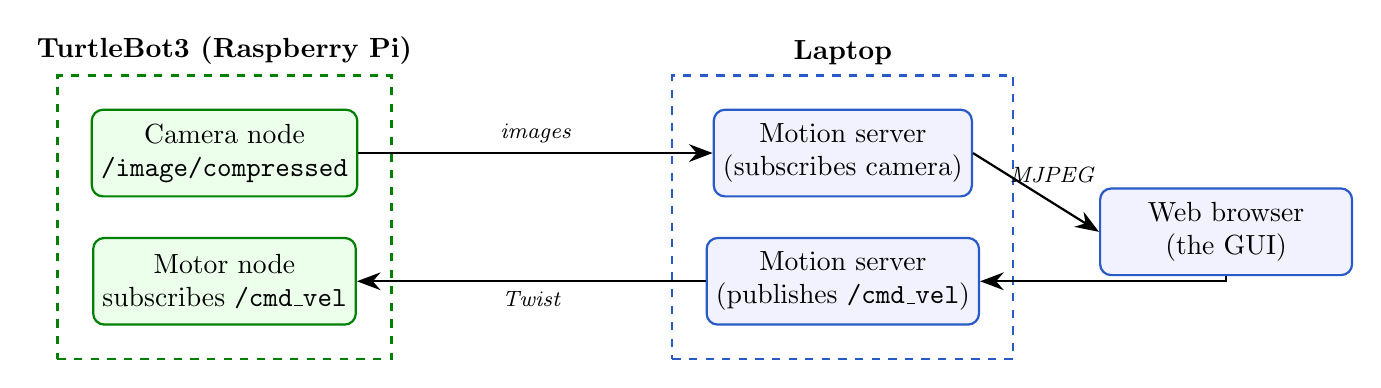
\begin{tikzpicture}[
  box/.style={rectangle, rounded corners, draw=accent, thick, fill=blue!5,
              minimum width=3.2cm, minimum height=1.1cm, align=center},
  robotbox/.style={rectangle, rounded corners, draw=green!50!black, thick,
              fill=green!8, minimum width=3.2cm, minimum height=1.1cm, align=center},
  arrow/.style={-{Stealth[length=3mm]}, thick},
  lbl/.style={font=\footnotesize\itshape}
]
% robot side
\node[robotbox] (cam) {Camera node\\\code{/image/compressed}};
\node[robotbox, below=0.5cm of cam] (motor) {Motor node\\subscribes \code{/cmd\_vel}};
\node[draw=green!50!black, thick, dashed, inner sep=12pt, fit=(cam)(motor),
      label=above:{\textbf{TurtleBot3 (Raspberry Pi)}}] (robot) {};

% laptop side
\node[box, right=4.5cm of cam] (sub) {Motion server\\(subscribes camera)};
\node[box, below=0.5cm of sub] (pub) {Motion server\\(publishes \code{/cmd\_vel})};
\node[box, right=1.6cm of sub, yshift=-1.0cm] (browser) {Web browser\\(the GUI)};
\node[draw=accent, thick, dashed, inner sep=12pt, fit=(sub)(pub),
      label=above:{\textbf{Laptop}}] (laptop) {};

% arrows
\draw[arrow] (cam.east) -- node[lbl, above]{images} (sub.west);
\draw[arrow] (pub.west) -- node[lbl, below]{Twist} (motor.east);
\draw[arrow] (sub.east) -- node[lbl, above, xshift=2mm]{MJPEG} (browser.west);
\draw[arrow] (browser.south) |- (pub.east);
\end{tikzpicture}
\caption{Data flow. Left: the robot. Right: the laptop. Camera images flow
right; drive commands flow left. Wi-Fi carries the ROS~2 traffic between them.}
\label{fig:arch}
\end{figure}

\noindent The two dashed boxes are the two computers. Inside the laptop, the
single \code{motion\_server.py} program plays several roles: it subscribes to the
camera, re-serves those frames to the browser as a video stream, and turns your
clicks into \code{/cmd\_vel} messages.

% ===========================================================================
\section{Hardware and Network Configuration}
% ===========================================================================
Table~\ref{tab:config} lists every setting the system depends on. All of these
live in a single \code{.env} file so they are easy to change (see
Appendix~\ref{app:env}).

\begin{table}[h]
\centering
\begin{tabular}{@{}lll@{}}
\toprule
\textbf{Setting} & \textbf{Value} & \textbf{Meaning} \\
\midrule
Robot IP        & \code{192.168.68.100} & Address of the robot on the Wi-Fi \\
Laptop IP       & \code{192.168.68.113} & Address of the laptop \\
Robot login     & \code{ubuntu}         & SSH username on the robot \\
ROS\_DOMAIN\_ID & \code{203}            & Shared ``channel group'' (Sec.~\ref{sec:domain}) \\
Robot model     & \code{burger}         & The TurtleBot3 variant \\
Lidar model     & \code{LDS-01}         & The distance sensor type \\
Camera topic    & \code{/image/compressed} & Where images are published \\
Command topic   & \code{/cmd\_vel}      & Where drive commands go \\
Max linear speed & \code{0.22} m/s      & Burger's top forward speed \\
Max angular speed & \code{2.84} rad/s   & Burger's top turning speed \\
Server port     & \code{8000}           & Web address is \code{localhost:8000} \\
\bottomrule
\end{tabular}
\caption{System configuration.}
\label{tab:config}
\end{table}

% ===========================================================================
\section{ROS 2 Topics and Interfaces Reference}
\label{sec:topics}
% ===========================================================================
Section~\ref{sec:domain} introduced topics as ``radio channels.'' This section
is the complete reference for the channels this robot actually broadcasts.

A point that confuses newcomers: \emph{topics are not defined in configuration
files.} There is no file you can open that lists them. A topic springs into
existence when a running node asks for it in code --- for example, the camera
node creates its channel with the single line

\begin{lstlisting}[language=Python]
self.publisher_ = self.create_publisher(CompressedImage, '/image/compressed', 1)
\end{lstlisting}

\noindent
(see \code{robot/.../image\_publisher.py}, line 38). So the authoritative list
of topics comes from asking the \emph{live} robot, not from reading a file.
Table~\ref{tab:topics} is exactly that: the output of \code{ros2 topic list} on
a running system, with each type resolved.

\begin{table}[h]
\centering
\small
\begin{tabular}{@{}lll@{}}
\toprule
\textbf{Topic} & \textbf{Message type} & \textbf{Published by} \\
\midrule
\code{/cmd\_vel}          & \code{geometry\_msgs/msg/Twist}        & \textbf{this app} (laptop $\to$ robot) \\
\code{/image/compressed}  & \code{sensor\_msgs/msg/CompressedImage}& \code{image\_publisher} (custom) \\
\code{/odom}              & \code{nav\_msgs/msg/Odometry}          & \code{diff\_drive\_controller} (read by \textbf{this app}) \\
\code{/scan}              & \code{sensor\_msgs/msg/LaserScan}      & \code{hlds\_laser\_publisher} \\
\code{/imu}               & \code{sensor\_msgs/msg/Imu}            & \code{turtlebot3\_node} \\
\code{/magnetic\_field}   & \code{sensor\_msgs/msg/MagneticField}  & \code{turtlebot3\_node} \\
\code{/battery\_state}    & \code{sensor\_msgs/msg/BatteryState}   & \code{turtlebot3\_node} \\
\code{/joint\_states}     & \code{sensor\_msgs/msg/JointState}     & \code{turtlebot3\_node} \\
\code{/sensor\_state}     & \code{turtlebot3\_msgs/msg/SensorState}& \code{turtlebot3\_node} \\
\code{/tf}, \code{/tf\_static} & \code{tf2\_msgs/msg/TFMessage}    & \code{robot\_state\_publisher} \\
\code{/robot\_description}& \code{std\_msgs/msg/String}            & \code{robot\_state\_publisher} \\
\bottomrule
\end{tabular}
\caption{Every topic on the running system (\code{ROS\_DOMAIN\_ID=203}).}
\label{tab:topics}
\end{table}

Of these eleven, the motion server touches exactly \textbf{three}: it subscribes
to \code{/image/compressed} for the video feed and to \code{/odom} to measure
distance and angle goals (Section~\ref{sec:closedloop}), and publishes to
\code{/cmd\_vel}. Everything else comes free with the standard bringup and is
there if you want to extend the project --- \code{/scan} for obstacle avoidance,
\code{/battery\_state} for a charge warning.

\subsection{Topics versus services}
A \textbf{topic} is one-way broadcast: the sender publishes and never learns who
listened. A \textbf{service} is a two-way request/response, like a phone call ---
you ask a question and wait for an answer.

Services \emph{are} defined in files, which is why the distinction matters here.
The robot package contains one, \code{srv/Motion.srv}, which declares a request
of two floats and a response of a success flag plus a message. It belongs to
the upstream Jetson AI stack and \textbf{is not used by this app} --- the web
GUI drives the robot purely by publishing \code{Twist} messages on
\code{/cmd\_vel}.

\subsection{Inspecting topics yourself}
\begin{lstlisting}[language=bash]
export ROS_DOMAIN_ID=203
ros2 topic list              # every topic currently on the network
ros2 topic type /cmd_vel     # what message type it carries
ros2 topic echo /odom        # print messages as they arrive
ros2 topic hz /scan          # measure how fast they arrive
ros2 node list               # which programs are running
\end{lstlisting}

\begin{warnbox}
If \code{ros2 topic list} shows only \code{/parameter\_events} and
\code{/rosout}, it is almost always a \textbf{stale ROS daemon}, not a network
fault --- and it will hide topics even on the robot itself. Fix it with
\code{ros2 daemon stop}, or add \code{-{}-no-daemon} to the command. Note that
\code{ros2 topic hz} does \emph{not} accept \code{-{}-no-daemon} on Humble: it
exits with a usage error that looks deceptively like ``no data.'' Discovery
also needs 20--30 seconds to fully settle after launch, so an incomplete list
immediately after starting the robot is normal.
\end{warnbox}

% ===========================================================================
\section{What Was Built: The Motion Server}
% ===========================================================================
The entire application is the file \code{motion\_server.py}. Here is what each
part does, in plain language.

\subsection{Camera streaming}
The server subscribes to the robot's camera topic. Each incoming compressed
image is decoded into a picture. A special web address, \code{/video}, streams
these pictures to the browser one after another (a technique called
\textbf{MJPEG}), which the browser shows as a live video. The program can handle
both ``raw'' and ``compressed'' image types and detects which one automatically.

\subsection{Driving the robot}
When you press a direction, the browser calls the address \code{/cmd} with a
requested linear and angular speed. The server clamps those numbers to the
robot's safe maximums and remembers them as the ``target velocity.''

\subsection{Safety: the dead-man's switch}
\label{sec:deadman}
A robot that keeps moving after you lose connection is dangerous. To prevent
this, the server re-sends the target velocity 20 times per second, but if no
fresh command has arrived in the last \textbf{0.4 seconds} it automatically
sends \emph{stop}. In practice this means: the robot moves only while you are
actively holding a button or key; the instant you release --- or your browser or
Wi-Fi drops --- it halts. This is called a \textbf{dead-man's switch}.

\subsection{The web GUI}
Figure~\ref{fig:gui} shows the interface. On the left is the live camera. On the
right is the control panel:
\begin{itemize}[noitemsep]
  \item A 3$\times$3 grid of labelled buttons: \emph{Forward, Backward, Turn
        Left, Turn Right}, the four diagonals, and a large red \textbf{STOP} in
        the centre.
  \item A live velocity read-out ($v$ and $\omega$).
  \item Sliders to set how fast forward driving and turning are.
  \item A latency read-out (explained in Section~\ref{sec:latency}).
\end{itemize}
You can also drive with the keyboard: \textbf{W/A/S/D} or the arrow keys, and
\textbf{Space} or \textbf{X} to stop. Press-and-hold to move; release to stop.

\begin{figure}[h]
\centering
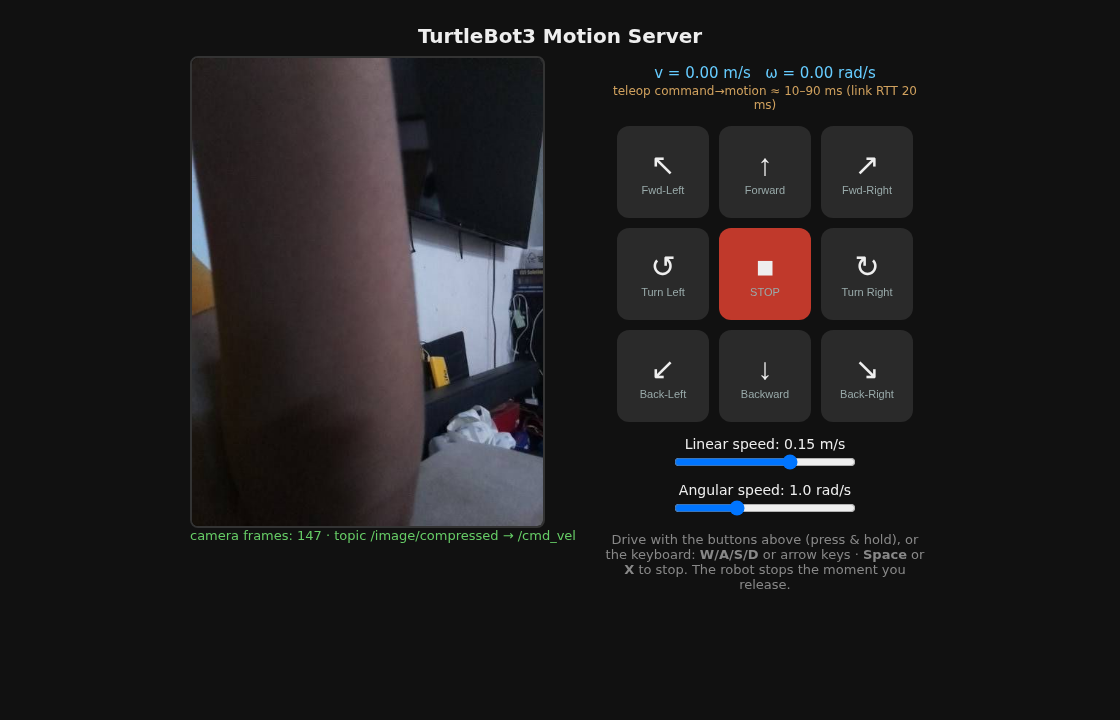
\includegraphics[width=\linewidth]{images/gui.png}
\caption{The web GUI. Camera feed on the left; full teleop control panel on the
right with directional buttons, STOP, speed sliders, and the latency read-out.}
\label{fig:gui}
\end{figure}

\subsection{Teleop latency read-out}
\label{sec:latency}
The amber line under the velocity read-out estimates how long it takes for a
button press to reach the robot as motion. It is built from a live measurement
of the network \textbf{round-trip time} plus fixed allowances for internal
processing --- see Section~\ref{sec:latencymath} for the full explanation.

% ===========================================================================
\section{Natural-Language Control with a Local LLM}
\label{sec:nl}
% ===========================================================================
Holding a key is precise but wordless. This section adds a second way to drive:
typing an instruction in plain English --- \emph{``move forward for 3 seconds''},
\emph{``move forward 1 meter''}, \emph{``rotate right 30 degrees''} --- and
having the robot carry it out. The language model runs \textbf{on the laptop}, so
no text ever leaves the machine.

An instruction can specify how \emph{long} to move, how \emph{far} to move, or
how far to \emph{turn}. The first is open-loop timing; the other two are
closed-loop and measured against the robot's odometry, which is the subject of
Section~\ref{sec:closedloop}. Several instructions can also be chained with
commas and run one after another --- Section~\ref{sec:chaining}.

\subsection{Why a typed command needs a timer}
This is the crux of the design, and it follows directly from the dead-man's
switch in Section~\ref{sec:deadman}. Holding a key works because the browser
sends a fresh command on every press; the robot keeps moving only while those
commands keep arriving, and stops 0.4\,s after they cease.

A typed instruction is a \emph{single event}. Send it once and the robot lurches
for 0.4\,s and dies. So a natural-language command is executed by a small
background worker that re-asserts the requested velocity every 0.1\,s for the
requested duration, then stops. It feeds the dead-man's switch deliberately,
for a bounded window.

Crucially, the dead-man's switch is left \emph{completely untouched} underneath.
If that worker thread crashes, or the whole server is killed mid-motion, no more
commands arrive and the robot halts within 0.4\,s anyway. The new feature sits
on top of the existing safety net rather than replacing it.

\subsection{The model only interprets; it never drives}
The model's sole job is to turn a sentence into a small, fixed record:

\begin{lstlisting}[style=py]
{"action": "forward", "mode": "distance", "value": 1, "speed": "normal"}
\end{lstlisting}

\noindent
\code{action} is restricted to six values (\code{forward}, \code{backward},
\code{rotate\_left}, \code{rotate\_right}, \code{stop}, \code{unknown}) by a JSON
schema enforced during decoding, so the model physically cannot emit anything
else. The result is then re-validated in Python and every number is clamped
before it can reach a motor.

\code{mode} tags what unit \code{value} carries: \code{duration} means seconds,
\code{distance} means metres, \code{angle} means degrees. One tagged number is
used rather than three separate optional fields, for a practical reason ---
under schema-constrained decoding an ``optional'' field is a coin flip, so all
three would end up mandatory, and a 3-billion-parameter model handed three
mutually exclusive numbers will dutifully fill in all of them, inventing a
duration for \emph{``move forward 1 meter''} purely because the slot exists.

The order of the fields in the schema is also deliberate. Decoders emit
properties in the order the schema lists them, so \code{mode} is placed
\emph{before} \code{value}: the model commits to the unit before it writes the
number. Reversed, it picks a number blind and then rationalises a unit for it.

That last step is not a formality. During development both candidate models were
asked to \emph{``drive forward for 3 hours''}: one returned a duration of
10\,800 seconds, the other 1\,800 seconds, and one of them classified it as a
perfectly ordinary drive command. Table~\ref{tab:nlsafety} lists the guards that
turn that into a harmless 10-second nudge.

\begin{table}[h]
\centering
\small
\begin{tabular}{@{}ll@{}}
\toprule
\textbf{Guard} & \textbf{Effect} \\
\midrule
Duration cap      & Clamped to \code{NL\_MAX\_DURATION} (default 10\,s) \\
Distance cap      & Clamped to \code{NL\_MAX\_DISTANCE} (default 2\,m) \\
Angle cap         & Clamped to \code{NL\_MAX\_ANGLE} (default 360\textdegree) \\
Chain budget      & Sequence refused over 5 steps / 3\,m / 720\textdegree{} / 120\,s \\
Chain aborts      & One failed step abandons every step after it \\
Mid-chain stop    & Refused; a \code{stop} must stand on its own \\
Speed clamp       & Velocities clamped to \code{MAX\_LIN} / \code{MAX\_ANG} \\
Fixed action list & Anything outside the six actions is refused \\
Auto-stop         & Every motion ends by itself; no ``drive forever'' \\
Goal timeout      & Closed-loop goals also carry a wall-clock deadline \\
Progress watchdog & $<$2\,mm or $<$1\textdegree{} for 1.5\,s aborts the motion \\
Odometry watchdog & \code{/odom} silent for 0.5\,s $\Rightarrow$ stop \\
No odometry       & Distance/angle refused outright, never estimated \\
STOP wins         & STOP, \textbf{Space} or \textbf{X} aborts a typed motion \\
Manual override   & \textbf{W/A/S/D} takes control from a running command \\
Dead-man backstop & Server dies mid-motion $\Rightarrow$ robot stops in 0.4\,s \\
Model unreachable & Falls back to a refusal, never to motion \\
\bottomrule
\end{tabular}
\caption{Safety guards on natural-language commands. All are enforced in code,
not by asking the model nicely.}
\label{tab:nlsafety}
\end{table}

\subsection{Distance and angle: measuring instead of guessing}
\label{sec:closedloop}
The speed sliders and a duration together imply a distance --- speed multiplied
by time. It is tempting to stop there: to turn \emph{``move forward 1 meter''}
into $1 \div 0.154 = 6.5$ seconds of driving and call it done. That is
\emph{open-loop} control, and it is wrong in a way that cannot be tuned out. The
robot accelerates rather than jumping to speed, the motors have a deadband, the
wheels slip, and a tired battery turns slower than a fresh one. Errors of
10--20\,\% are normal, and nothing in the loop ever notices.

Instead the server subscribes to \code{/odom}, the odometry the robot already
publishes 20 times a second, and \emph{measures}. For a distance goal it records
the starting position and watches the straight-line displacement grow; for an
angle goal it watches the heading. When the remaining error falls inside a
tolerance band, it stops.

\subsubsection{Easing into the goal}
A na\"ive version --- drive at full speed until the goal is reached, then stop
--- overshoots badly, and the reason is worth spelling out. Between the instant
the robot is actually at the goal and the instant its wheels stop, the following
must happen: the next odometry sample has to arrive (up to 50\,ms), cross the
Wi-Fi (5--20\,ms), be noticed by the control loop (up to 50\,ms), be published on
the next command tick (up to 50\,ms), cross back, and finally be acted on by the
motors (30--80\,ms). That is roughly \textbf{150\,ms} of unavoidable lag. At
normal speed the robot travels 2\,cm --- or turns \textbf{17\textdegree} --- in
that time.

The fix is to slow down before arriving. The commanded speed is scaled down
proportionally over the last 10\,cm (or 25\textdegree), so by the time the stop
decision is made the robot is already crawling, and 150\,ms of lag costs
millimetres instead of centimetres.

There is a floor under that ramp, and it matters: a TurtleBot3 below roughly
0.01\,m/s simply buzzes without moving. The commanded speed is never allowed
below about twice that. This produces a genuine tension --- a higher floor
overshoots, a lower one stalls short of the goal and burns the timeout --- and it
is the floor, not the tolerance, that ultimately bounds the error.

\subsubsection{Turning past half a circle}
Odometry reports heading as an angle between $-\pi$ and $+\pi$, which wraps.
Subtracting a start heading from a current one na\"ively means a
270\textdegree{} turn appears to fold back on itself and the goal is never
reached --- the robot would spin until the timeout. So each incoming sample's
\emph{change} in heading is unwrapped and accumulated into a running total that
is free to pass $\pi$. At 20\,Hz the largest genuine change between samples is
about 0.14\,rad, far from the $\pi$ boundary, so the correction is never
ambiguous. A jump larger than 2\,rad is not a rotation at all but an odometry
reset, and is flagged as such rather than silently corrupting the total.

\subsubsection{Why this cannot mean ``drive forever''}
Section~\ref{sec:deadman} promised that every motion ends by itself. A goal that
stops when the robot \emph{arrives} threatens exactly that promise, because a
robot that cannot arrive would never stop. Three independent endings are
therefore in place: reaching the goal; a progress watchdog that aborts after
1.5\,s of no measurable movement; and a wall-clock timeout of roughly three
times the ideal duration plus a margin. The 0.4\,s dead-man's switch sits
underneath all three.

\begin{warnbox}
None of these watchdogs catches a robot that has been \emph{picked up}.
TurtleBot3 odometry comes from wheel encoders, so wheels spinning in the air
report flawless progress and a lifted robot will cheerfully ``complete'' a
1-metre move. The watchdogs catch \emph{blocked} and \emph{odometry-dead}, not
\emph{airborne}. This is a real limitation --- and, conveniently, what makes
testing on blocks so effective.
\end{warnbox}

\subsubsection{How accurate is it?}
Expect about \textbf{$\pm$2\,cm and $\pm$5\textdegree} on a hard floor; carpet is
worse. Note carefully what that is measured against: the robot's own wheel
odometry, which itself drifts 1--3\,\% through slip. It is \emph{not} a claim
about absolute heading. Over a full 360\textdegree{} spin, odometry may report
exactly 360.0 while the true heading is several degrees off. Tuning the
tolerances to compensate for slip would be a mistake --- that is a calibration
problem, not a control problem.

\subsection{Chaining several instructions}
\label{sec:chaining}
Commas (or \emph{then}, or semicolons) join instructions into a sequence, run
strictly in order, each beginning only once the previous one has finished:

\begin{lstlisting}[style=bash]
move forward 0.5 m, turn right 90 degrees, move forward 0.3 m
\end{lstlisting}

\subsubsection{Splitting happens before the model, not inside it}
The obvious approach --- ask the model for a \emph{list} of steps --- is the
wrong one here. The text is split into clauses in Python and each clause is sent
to the model on its own, for three reasons.

The decisive one is that failures stay \textbf{attributable}. Holding the
fragment lets the server say \emph{step 2 of 3 (``go to the kitchen''): not a
driving command I understand}. Had the model chosen the decomposition, there
would be no span of the user's own words to quote back at them.

Second, the prompt and schema from the previous section are left untouched, so
the single-instruction behaviour they were tested against is unchanged by
construction rather than by hope. Third, under schema-constrained decoding the
\emph{length} of an array is not reliably constrained, so a step limit would
become a check applied after the fact to however many steps the model felt like
emitting, instead of a property of the user's own punctuation.

The splitter has one subtlety worth stating: a fragment containing no movement
word is treated as a \emph{qualifier} and glued back onto its neighbour. This is
what keeps \emph{``move forward 1 m, slowly''} a single instruction. Note also
that a bare \emph{and} is deliberately not a separator --- \emph{``go forward a
meter and a half''} must survive intact.

\subsubsection{One thread, one cancel}
The whole sequence runs on a single worker thread sharing a single cancellation
flag. This is a safety property, not a tidiness one.

The tempting alternative --- let each step, as it finishes, launch the next ---
races the STOP path. Stopping works by raising the cancel flag and then waiting
briefly for the worker to exit. If a dying worker spawns its successor, that
wait can return with a \emph{brand new} motion already running, and the robot
carries on. The STOP button would appear to do nothing. Keeping the whole
sequence inside one cancellable worker means the existing STOP button, the
keyboard, and a typed \emph{halt} all abort the entire sequence without any of
them needing to know that sequences exist.

\subsubsection{A failed step abandons the rest}
If any step ends for any reason other than reaching its goal --- timeout,
blocked wheels, odometry loss, the STOP button --- the remaining steps are
discarded rather than attempted.

This is the whole reason the feature needs care. Suppose \emph{``forward 0.5 m,
turn right 90\textdegree, forward 0.3 m''} and the turn stops at 41\textdegree.
Carrying on would drive the final leg 49\textdegree{} away from where it was
meant to go --- confidently, and in a direction nobody asked for. A sequence is
only meaningful while every step before it did what it said.

\subsubsection{The pause between steps}
Steps are separated by a deliberate 0.35\,s pause with zero velocity commanded
explicitly. It is not there for braking --- the ramp of
Section~\ref{sec:closedloop} hands off at the speed floor, so the robot is
physically stopped in well under 50\,ms.

It is there because the \emph{measurement} lags the robot. Odometry is the last
sample \emph{received}, up to a 20\,Hz period plus wireless transport old. A step
that snapshots its starting pose while the robot is still moving measures its
goal from a position the robot has already left. The pause lets several fresh
samples arrive after the robot is genuinely still. It is also kept below the
0.4\,s dead-man's timeout, so a healthy sequence never relies on that backstop.

\subsubsection{Budgets for the whole sequence}
Every cap in Table~\ref{tab:nlsafety} was per \emph{motion}. Three steps of two
metres each would clear all of them individually and drive six metres. A
sequence therefore carries its own budget --- 5 steps, 3\,m of path, 720\textdegree,
120\,s worst case --- and is \textbf{refused} rather than trimmed when it
exceeds one.

Refusing breaks symmetry with the per-step caps on purpose. A capped step has a
repair the user can see in their own sentence (``capped from 5\,m''). Trimming a
sequence to fit has no such reading: which step should lose out? The result
would be a robot ending up somewhere the user could not have predicted from what
they typed.

Note the distance budget bounds \emph{path length}, not displacement:
\emph{``forward 2 m, backward 2 m''} spends 4\,m of it and finishes where it
started. For a room-sized safety argument, path length is the right thing to
bound.

\begin{warnbox}
\textbf{Chaining is sequential convenience, not a path-accurate trajectory.}
Each step measures from where the robot \emph{believes} it is when that step
starts, so errors compound: a 5\textdegree{} heading error left over from one
turn rotates the whole of the next leg's displacement, putting a 0.3\,m leg
about 2.6\,cm off to the side, and it grows with the length of the sequence.
Four 90\textdegree{} turns will not reliably close a square. A path the robot
genuinely follows needs a map and a localiser; this is dead reckoning with good
manners.
\end{warnbox}

\subsection{What it costs you}
Parsing takes roughly \textbf{2--4 seconds} on an RTX 3060 with
\code{qwen2.5:3b} --- the delay between pressing Enter and the robot moving. The
first command after an idle period can take around 16 seconds while the model is
loaded into memory; the server passes \code{keep\_alive} to ollama to avoid
paying that repeatedly. For reflex-speed driving, keep using the keyboard; this
is a different, more conversational way to work.

\subsection{Trying it without moving the robot}
The \code{/nl} endpoint accepts \code{?dry\_run=1}, which parses and clamps the
instruction and reports what \emph{would} happen, without sending any motion
command. This is the safe way to check the model's understanding:

\begin{lstlisting}[style=bash]
curl -s -X POST 'http://localhost:8000/nl?dry_run=1' \
     -H 'Content-Type: application/json' \
     -d '{"text":"move forward 5 meters"}'
# -> {"action":"forward","mode":"distance","value":2.0,"capped":true, ...}
\end{lstlisting}

\noindent
Dry runs work with the robot switched off entirely, so phrasings can be
developed without it. A second server started on a command topic the robot does
not subscribe to is inert in a different and useful way:

\begin{lstlisting}[style=bash]
python3 motion_server.py --cmd-vel-topic /cmd_vel_test --port 8001 \
        --image-topic /nonexistent --image-type raw --enable-nl
\end{lstlisting}

\noindent
Nothing moves, but \code{/odom} is real --- so every closed-loop goal ends in the
progress watchdog. That is not a limitation of the test, it \emph{is} the test:
it proves the backstops fire, and it times them.

For chained commands this instance is more useful still. An all-duration
sequence is open-loop, so it \emph{runs to completion} with the robot standing
still --- a genuine end-to-end test of the sequencing, in which the total elapsed
time also confirms that the pause between steps really happened. Mixing in a
single distance or angle step then produces a real mid-sequence failure, which
is how you check that the steps after it are abandoned rather than attempted.

\begin{warnbox}
Natural language is a convenience layer, not an autonomy layer. The robot has no
idea what is in front of it --- there is no obstacle avoidance on this path. It
will happily drive into a wall if you ask it to. Keep watching the robot, keep a
hand near STOP, and test with the wheels off the ground first.
\end{warnbox}

% ===========================================================================
\section{Problems Encountered and How They Were Solved}
\label{sec:fixes}
% ===========================================================================
Getting the system working surfaced several real-world issues. They are
documented here because they are common and instructive.

\begin{description}
  \item[Nothing was visible at first.] The robot was powered on but its ROS
        software had not been started. Powering on a robot is not the same as
        launching its programs --- the motor and camera nodes must be started
        explicitly.
  \item[Domain ID mismatch.] The robot's start-up file (\code{.bashrc}) set the
        ROS\_DOMAIN\_ID \emph{five} times with conflicting values; the last one
        won, leaving the robot on domain 0 while the laptop was on 203. Because
        of the rule in Section~\ref{sec:domain}, they could not see each other.
        The file was cleaned to set a single, consistent value (203).
  \item[Missing lidar model.] Launching the robot failed with
        \code{KeyError: 'LDS\_MODEL'} because the lidar type was not set in the
        environment. Setting \code{LDS\_MODEL=LDS-01} fixed it.
  \item[SSH dropping on launch.] Every time the robot software started, the
        remote terminal connection reset (a Wi-Fi hiccup under the sudden burst
        of network traffic). The fix was to launch the robot programs
        \emph{detached}, so they keep running even if the terminal disconnects.
  \item[Multicast worry.] The home Wi-Fi (a \code{192.168.68.x} network, typical
        of Google/Nest routers) was suspected of blocking the ``multicast''
        traffic ROS uses to discover nodes. A unicast fall-back configuration
        (\code{fastdds\_unicast.xml}) was prepared, but testing showed multicast
        actually worked, so the default is used.
\end{description}

% ===========================================================================
\section{How to Run Everything}
% ===========================================================================
This is the complete operating procedure.

\subsection{One-time setup}
\begin{lstlisting}[style=bash]
# Copy the configuration template and fill in your values
cp .env.example .env
nano .env        # set ROBOT_IP, ROBOT_PASSWORD, ROS_DOMAIN_ID, etc.
\end{lstlisting}

\subsection{Step 1 --- Start the robot's software}
This starts the motor driver and the camera on the robot, over SSH:
\begin{lstlisting}[style=bash]
./scripts/robot_start.sh
\end{lstlisting}
It launches everything on the correct domain and waits for it to come up. You can
confirm the robot's topics are visible from the laptop with:
\begin{lstlisting}[style=bash]
export ROS_DOMAIN_ID=203
ros2 topic list        # you should see /cmd_vel, /image/compressed, /scan, ...
\end{lstlisting}

\subsection{Step 2 --- Start the web server}
\begin{lstlisting}[style=bash]
./run_server.sh
\end{lstlisting}

\subsection{Step 3 --- Open the GUI and drive}
Open \url{http://localhost:8000} in a browser (or
\code{http://192.168.68.113:8000} from your phone on the same Wi-Fi). Drive with
the buttons or keyboard. \emph{Watch the robot while you drive.}

\subsection{Step 4 --- Shut down}
\begin{lstlisting}[style=bash]
# Stop the web server:  press Ctrl-C in its terminal, or:
pkill -f motion_server.py

# Stop the robot's ROS nodes (robot stays powered on):
./scripts/robot_stop.sh
\end{lstlisting}

\subsection{Step 5 --- Power off the robot (optional)}
Always shut the Raspberry Pi down cleanly before cutting power, to avoid
corrupting its memory card:
\begin{lstlisting}[style=bash]
ssh ubuntu@192.168.68.100 'sudo poweroff'
# wait ~20 s for the green light to stop blinking, then flip the power switch
\end{lstlisting}

% ===========================================================================
\section{Understanding Teleop Latency}
\label{sec:latencymath}
% ===========================================================================
\textbf{Latency} is the delay between doing something and seeing the effect.
For teleop, it is the time from pressing a button to the wheels actually turning.

The most important and variable part is the \textbf{Round-Trip Time (RTT)}: how
long a small network packet takes to travel from the laptop to the robot
\emph{and back}. The server measures this live (it appears as ``link RTT'' in the
GUI). A typical value on this setup is about 20\,ms; if the Wi-Fi degrades, this
number climbs and driving feels sluggish.

A command only needs to travel \emph{one way} (laptop $\rightarrow$ robot), which
is about half the RTT. The GUI's estimate therefore adds up:
\[
\text{latency} \;\approx\;
\underbrace{\tfrac{1}{2}\,\text{RTT}}_{\text{network, one way}}
\;+\;
\underbrace{50\,\text{ms}}_{\text{command cycle (20 Hz)}}
\;+\;
\underbrace{\sim 30\,\text{ms}}_{\text{motor response}}.
\]
For a 20\,ms RTT this gives roughly 10--90\,ms. Note this is a well-grounded
\emph{estimate}: only the RTT is measured directly; the other terms are known
constants of the system.

% ===========================================================================
\section{Troubleshooting}
% ===========================================================================
\begin{table}[h]
\centering
\begin{tabular}{@{}p{5.3cm}p{8.5cm}@{}}
\toprule
\textbf{Symptom} & \textbf{Likely cause and fix} \\
\midrule
\code{ros2 topic list} shows nothing from the robot &
Robot software not started (run \code{robot\_start.sh}), or domain mismatch
(both must be \code{ROS\_DOMAIN\_ID=203}). \\
GUI says ``waiting for camera'' but the robot drives &
Wrong camera topic; check \code{ros2 topic list} and \code{IMAGE\_TOPIC} in \code{.env}. \\
Camera shows but robot will not move &
Wrong command topic, or the robot's motor node is not running. \\
Robot launch fails: \code{KeyError: 'LDS\_MODEL'} &
Set \code{LDS\_MODEL} (e.g.\ \code{LDS-01}) before launching. \\
SSH disconnects when starting the robot &
Expected Wi-Fi hiccup; the scripts launch detached so the nodes survive. Just
reconnect and check. \\
Driving feels laggy &
Check the ``link RTT'' in the GUI; a high value means poor Wi-Fi. \\
\bottomrule
\end{tabular}
\caption{Common problems.}
\end{table}

% ===========================================================================
\section{Repository Structure and Security}
% ===========================================================================
\begin{lstlisting}[style=bash]
ttb-experiments/
  motion_server.py          # the whole application (node + server + GUI)
  run_server.sh             # start the server on the laptop (reads .env)
  scripts/
    robot_start.sh          # start the robot's ROS nodes over SSH
    robot_stop.sh           # stop the robot's ROS nodes
  fastdds_unicast.xml       # optional fall-back for multicast-blocking networks
  .env.example              # configuration template (safe to share)
  .env                      # YOUR real config incl. password (git-ignored!)
  robot/                    # reference snapshot of the ROBOT-side files
    start_all.sh            #   launches bringup + camera on the robot
    turtlebot3_image_motion/
      turtlebot3_image_motion/image_publisher.py  # the camera node
      srv/Motion.srv        #   a service definition (unused by this app)
      package.xml / CMakeLists.txt
  docs/
    turtlebot3_motion_server.tex / .pdf   # this document
    images/gui.png
\end{lstlisting}

\paragraph{About \code{robot/}.} Those files run on the robot, not the laptop,
and are copied here only so this repository documents the whole system. They are
a snapshot of commit \code{54fb8a2} of a separate project,
\url{https://github.com/SuperMadee/AI361-MEX3}, which remains the source of
truth --- the robot builds from its own clone in \code{\textasciitilde/ros2\_ws},
so editing the copies here changes nothing on the robot. Only the parts this
project depends on were copied; the upstream package's Jetson-side AI stack
(roughly 15{,}000 lines) is deliberately not duplicated.

\paragraph{Security note.} The robot's SSH password and other real values live
only in \code{.env}, which is listed in \code{.gitignore} and is therefore
\emph{never} committed or pushed to GitHub. Only \code{.env.example}, containing
placeholders, is shared. Never put real passwords in a public repository ---
automated bots scan GitHub for leaked credentials within minutes.

% ===========================================================================
\appendix
\section{Environment Variable Reference}
\label{app:env}
% ===========================================================================
\begin{table}[h]
\centering
\begin{tabular}{@{}ll@{}}
\toprule
\textbf{Variable} & \textbf{Description} \\
\midrule
\code{ROBOT\_IP}        & Robot's IP address on the Wi-Fi. \\
\code{LAPTOP\_IP}       & Laptop's IP address. \\
\code{ROBOT\_USER}      & SSH username on the robot. \\
\code{ROBOT\_PASSWORD}  & SSH password (secret; kept only in \code{.env}). \\
\code{ROS\_DOMAIN\_ID}  & Shared discovery domain; must match on both machines. \\
\code{TURTLEBOT3\_MODEL}& Robot variant (\code{burger}). \\
\code{LDS\_MODEL}       & Lidar model (\code{LDS-01}). \\
\code{IMAGE\_TOPIC}     & Topic the camera publishes on. \\
\code{IMAGE\_TYPE}      & \code{compressed}, \code{raw}, or \code{auto}. \\
\code{CMD\_VEL\_TOPIC}  & Topic drive commands are published on. \\
\code{ODOM\_TOPIC}      & Odometry topic read to measure distance/angle goals. \\
\code{MAX\_LIN}         & Max linear speed (m/s). \\
\code{MAX\_ANG}         & Max angular speed (rad/s). \\
\code{SERVER\_PORT}     & Web server port. \\
\code{ENABLE\_NL}       & \code{1} to enable natural-language driving (Sec.~\ref{sec:nl}). \\
\code{LLM\_URL}         & ollama base URL (default \code{http://localhost:11434}). \\
\code{LLM\_MODEL}       & Model used to parse commands (\code{qwen2.5:3b}). \\
\code{NL\_MAX\_DURATION}& Hard cap in seconds on any single typed motion. \\
\code{NL\_MAX\_DISTANCE}& Hard cap in metres on any single typed distance goal. \\
\code{NL\_MAX\_ANGLE}   & Hard cap in degrees on any single typed angle goal. \\
\code{GOAL\_TIMEOUT\_MAX}& Ceiling in seconds on a closed-loop goal's timeout. \\
\code{NL\_MAX\_STEPS}   & Most steps allowed in one chained sequence. \\
\code{NL\_MAX\_CHAIN\_DISTANCE}& Cap in metres on total path length per sequence. \\
\code{NL\_MAX\_CHAIN\_ANGLE}& Cap in degrees on total rotation per sequence. \\
\code{NL\_MAX\_CHAIN\_SECONDS}& Cap on a sequence's worst-case running time. \\
\bottomrule
\end{tabular}
\end{table}

\section{Command Cheat-Sheet}
\begin{lstlisting}[style=bash]
# --- laptop ---
./run_server.sh                       # start the web GUI server
pkill -f motion_server.py             # stop it
export ROS_DOMAIN_ID=203; ros2 topic list   # what the robot is publishing

# --- robot (over SSH) ---
./scripts/robot_start.sh              # start motors + camera
./scripts/robot_stop.sh              # stop them
ssh ubuntu@192.168.68.100 'sudo poweroff'    # clean power-off
\end{lstlisting}

\end{document}
